\section{Задание 1. Дифференциальные модели первого порядка}

\textbf{Условие.}

В задачах проведите исследование:

\begin{enumerate}
    \item Составьте математическую модель задачи: введите обозначения, выпишите данные, в задаче B сделайте чертеж, составьте дифференциальное уравнениеи запишите начальные условия.
    \item Решите аналитически составленную задачу Коши.
    \item Изобразите семейство интегральных кривых и решение задачи Коши.
    \item Запишите ответ
\end{enumerate}

\begin{enumerate}[label=\Alph*.]
    \item В электрическую цепь с сопротивлением $3/2$ Ом в течение двух минут равномерно вводится напряжение (от нуля до $120$ В).
    Кроме того, автоматически вводится индуктивность, так что число, выражающее индуктивность цепи в генри, равно числу,
    выражающему ток в амперах.
    Найдите зависимость тока от времени в течение первых двух минут опыта.

    \item Найти такую кривую, проходящую через точку $(0, -2)$, чтобы угловой коэффициент касательной в любой ее точке равнялся
    ординате этой точки, увеличенной на три единицы
\end{enumerate}

\vspace{10mm}
\textbf{Решение.}

\begin{enumerate}[label=\Alph*.]
    \item Пусть $U(t) = \frac{120}{2 \cdot 60}t = t$ - напряжение в цепи, $I(t)$ - сила тока в цепи, $R = \frac{3}{2}$ - сопротивление цепи.

    Катушка с индуктивностью $L = I(t)$ в цепи будет создавать магнитный поток $\Phi = LI = I^2(t)$ и
    ЭДС самоиндукции $\varepsilon(t) = -L\frac{dI(t)}{dt} = -I(t)\frac{dI(t)}{dt}$, направленный в противоположную сторону.

    Воспользуемся законом Ома:

    \[U(t) + \varepsilon(t) = I(t)R\]

    \[t = I(t)\frac{3}{2} + I(t)\frac{dI(t)}{dt}\]

    \[t - I(t)\frac{3}{2} = I(t)\frac{dI(t)}{dt}\]

    \[\frac{t - I(t)\frac{3}{2}}{I(t)} = \frac{dI(t)}{dt}\]

    Воспользуемся заменой $y = \frac{I(t)}{t}, I^\prime(t) = \frac{dI(t)}{dt} = \frac{d(yt)}{dt} = y^\prime t + y$:


    \[\frac{2 - 3y}{2y} = y^{\prime} t + y\]

    \[\frac{2 - 3y - 2y^{2}}{2y} = y^{\prime} t\]

    \[\frac{2ydy}{2 - 3y - 2y^{2}} = \frac{dt}{t}\]

    \[\frac{2ydy}{(y + 2)\left(2y - 1\right)} = -\frac{dt}{t}\]

    \[\frac{y}{(y + 2)\left(2y - 1\right)} = \frac{A}{y + 2} + \frac{B}{2y - 1} = \frac{2Ay - A + By + 2B}{(y + 2)(2y - 1)} \Longleftrightarrow \begin{cases}A = \frac{2}{5} \\ B =\frac{1}{5}\end{cases}\]

    \[2\int \frac{ydy}{(y + 2)(2y - 1)} = \frac{4}{5} \int \frac{dy}{y + 2} + \frac{1}{5} \int \frac{d2y}{2y - 1} = -\ln |t| + C\]

    \[\frac{4}{5} \ln |y + 2| + \frac{1}{5} \ln |2y - 1| = -\ln |t| + C\]

    \[\left(\sqrt[5]{y + 2}\right)^4 \sqrt[5]{2y - 1} = \frac{C}{t}\]

    \[(y + 2)^4 (2y - 1) = \frac{C}{t^5}\]

    \[\left(\frac{I(t)}{t} + 2\right)^4 \left(2\frac{I(t)}{t} - 1\right) = \frac{C}{t^5}\]

    \[(I(t) + 2t)^4 (2I(t) - t) = C\]


    Так как в начале опыта напряжения в токе не было, при $t_0 = 0$ сила тока $I(t_0) = 0$, поэтому $C = 0$, получаем решение $(I(t) + 2t)^4 (2I(t) - t) = 0$

    График семейства интегральных кривых (отмеченных синим) и решения задачи Коши (отмеченного красным):

    \begin{center}
        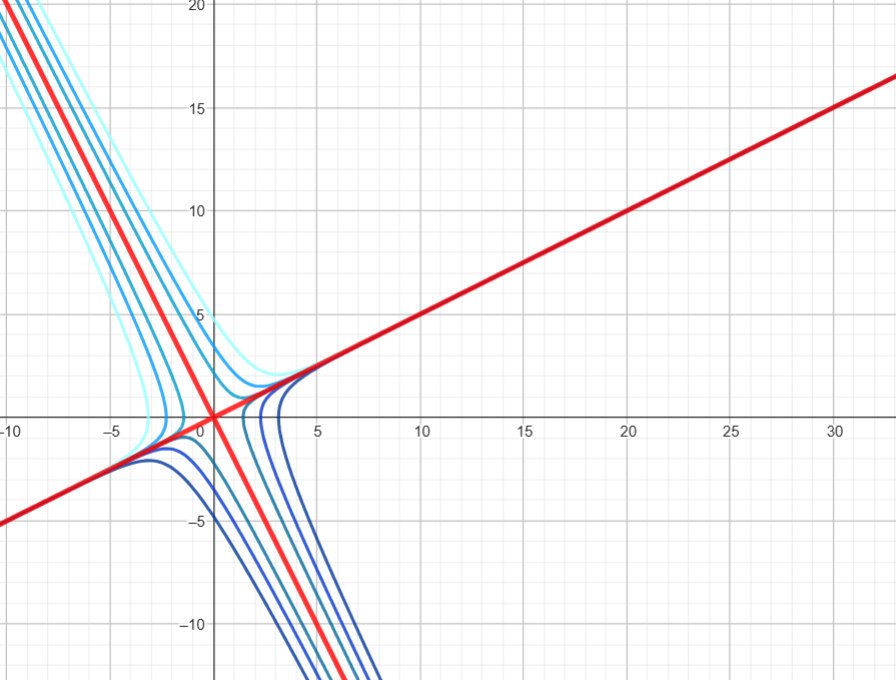
\includegraphics[height=80mm]{images/1a1}
    \end{center}

    \vspace{10mm}

    \item Зная, что угловой коэффициент касательной равняется утроенной ординате, можем сказать, что:

    \[y^\prime = 3y\]

    \[\frac{dy}{dx} = 3y\]

    \[\frac{dy}{y} = 3dx\]

    \[\ln |y| = 3x + C\]

    \[y = Ce^{3x}\]

    Начальным условием является $y(0) = -2$, поэтому $C = \frac{y}{e^{3x}} = \frac{-2}{1} = -2$, решением задачи Коши является $y = -2e^{3x}$

    График семейства интегральных кривых (отмеченных синим) и решения задачи Коши (отмеченного красным):

    \begin{center}
        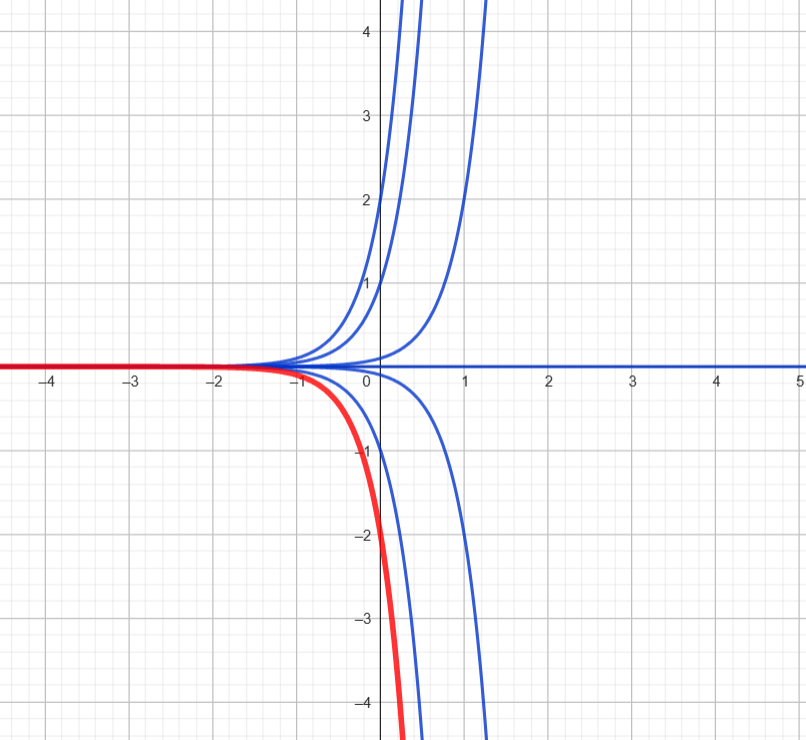
\includegraphics[height=80mm]{images/1b1}
    \end{center}


\end{enumerate}

